\chapter{Erweiterte Funktionalitäten}
In diesem Kapitel werden nun weitere Funktionen beschrieben, die über die Grundausstattung der Web-App und die WebSockets hinausgehen, um die Arbeit zu erweitern und produktiver zu gestalten. 

%%%%%%%%%%%%%%%%%%%%%%%%%%%%%%%%%%%%%%%%%%%%%%%%%%

\section{Lokalisierung von Clients}
Mit HTML5 wurde die \emph{navigator.geolocation} Klasse in die JavaScript API eingebaut. Diese Klasse ermöglicht es einer Webanwendung die Position des Anwenders zu erhalten - aber nur, wenn der Anwender zustimmt. Das geschieht bei aktuellen Smartphones unter Anderem mit in der Umgebung befindlichen WLAN Netzwerken, deren Standorte in einer Datenbank gespeichert sind. Verfügt das Gerät über GPS, so werden diese Daten auch berücksichtigt und ermöglichen eine genauere Ortung \cite[1. Absatz]{html5:geolocations}.

\paragraph{Koordinieren von Helfern}
Um die eingetragenen Helfer in dieser Webanwendung besser koordinieren zu können, wurde daher ein Skript implementiert, welches im Hintergrund der Web-App läuft und die aktuelle Position des Endgeräts über eine SSL verschlüsselte Verbindung an den Server übermittelt. Unter der Voraussetzung, dass der Client diesem Vorgang zustimmt sind dem Server damit die Positionen der eingeloggten Benutzer bekannt. Diese Positionsdaten können dann von der Anwendung ausgewertet und in einer Karte von \emph{Google Maps} \cite{google:maps} visualisiert werden.

\begin{figure}[!ht]
	\centering
	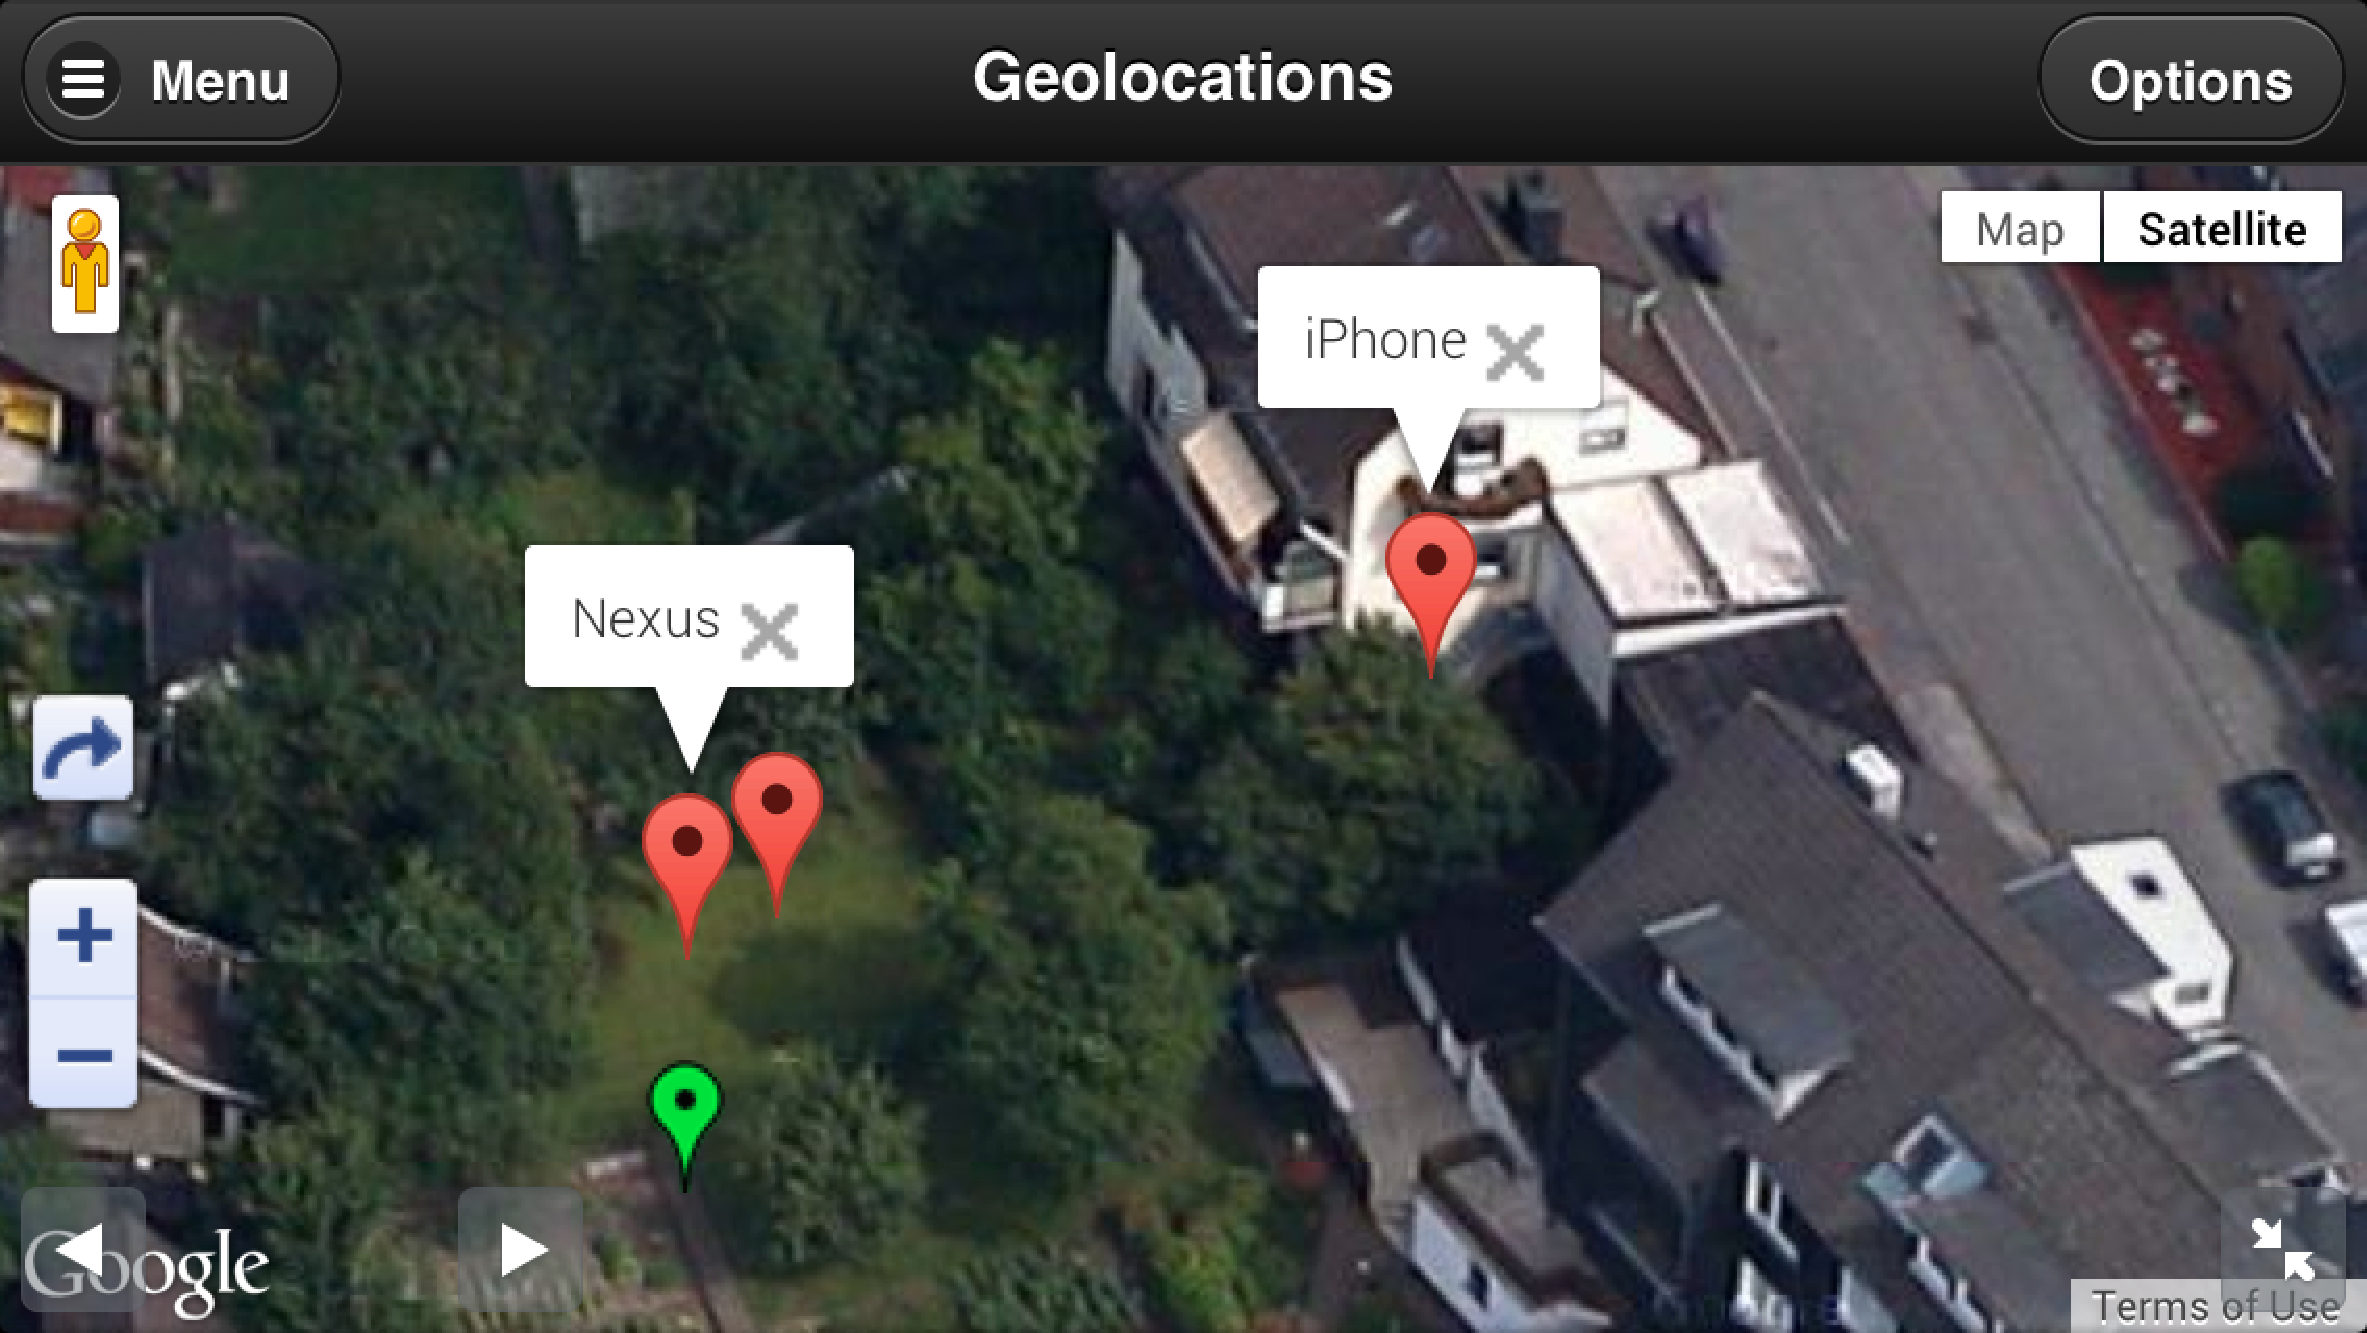
\includegraphics[width=15cm]{fig/screenshot_geolocations}
	\caption[Beispielansicht der Geolocations]{Getestet unter iOS 6.1.4, iPhone 5, Safari: Grün markiert eigene Position. Durch Tippen auf andere Marker erscheint der Name des Benutzers}
\end{figure}

Jeder Client kann auf diese Weise die Positionen der anderen Helfer sehen. Der Vorteil liegt klar auf der Hand: eine zentral eingerichtete Verwaltung kann mit einem Blick sehen, wer sich an welcher Stelle auf dem Gelände befindet. So können Wege optimiert und gezielt Aufgaben an sogenannte Springer verteilt werden, da ortsnahe Helfer die entsprechenden Aufgaben übernehmen können. Die kurzen Wege sorgen dann dafür, dass eine höhere Nutzung der Ressourcen (hier: die Helfer) möglich ist.\par

\paragraph{Anforderungen}
Eine wichtige Anforderung an diese Funktion ist, dass die Daten schnell ausgetauscht werden. Wenn zwischen den Updates der Geolocations zu viel Zeit vergeht, ist die Position nicht mehr aktuell und damit nicht mehr relevant. Deswegen findet der Austausch von Longitude und Latitude auch über WebSockets statt.\\
Damit ein Client die Positionen der anderen Teilnehmer erhält, muss er seine eigene Position an den WS Server schicken oder auf eine Aktualisierung der anderen Benutzer warten. Mit jedem \emph{locations}-Paket, welches an den Server geschickt wird, werden die aktualisierten Positionen an alle verbundenen Geräte verschickt. Das bedeutet auch, dass ein Client ohne WebSockets-Unterstützung keine Informationen über die Standorte erhält.

\paragraph{Kein Speichern der Positionsdaten}
Beendet ein Client die Verbindung oder erhält der Server keine Aktualisierungen mehr, so wird sein letzter Standort noch 15 Minuten gespeichert und dann auf allen Endgeräten gelöscht. Zu keiner Zeit werden Daten protokolliert oder länger als nötig aufbewahrt.

\paragraph{Automatische Berechnung der Ansicht der Karte}
Die Zoomstufe und Zentrierung der Google Maps Karte wird automatisch berechnet, wenn der Benutzer das möchte. Dabei werden alle Koordinaten in eine Variable geschrieben und der Mittelwert gebildet, um so einen Punkt für die Zentrierung zu finden. Über die Methode \emph{fitbounds(LatLngBounds)}, die von der Google API bereitgestellt wird, wird die optimale Zoomstufe berechnet. So wird die Karte immer so positioniert, dass sie alle Marker angepasst anzeigt.

\subsection{Umgebungsbedingte Einschränkungen}
Bei diesem Projekt handelt es sich um eine Webanwendung, die aufgrund von Sicherheitsvorkehrungen einigen Einschränkungen unterliegt. So erlauben die mobilen Betriebssysteme keine Geopositionierung durch den Browser, wenn dieser minimiert ist oder das Smartphone / Tablet nicht aktiv genutzt wird. Das bedeutet, dass die Meißner App geöffnet sein muss, damit alle Funktionen genutzt und aktualisiert werden können.\par

Das ist für die Lokalisierung problematisch, da so die Position des Clients nicht aktuell bleibt. Diese Sicherheitsmaßnahmen sind jedoch sehr sinnvoll, denn es wäre sehr bedenklich könnte eine Homepage im Hintergrund stetig die Position des Besuchers überwachen. Der Stromverbrauch wäre auch sehr hoch bei dauerhaftem GPS Signal. Allerdings genügt es, wenn die Webanwendung in einem Tab geöffnet ist, welcher nicht aktiv sein muss, um die Position des Endgeräts zu erfahren.

%%%%%%%%%%%%%%%%%%%%%%%%%%%%%%%%%%%%%%%%%%%%%%%%%%

\section{Offline-Funktionalität}
Mit der HTML5-Spezifikation wurde die \emph{Application Cache API} eingeführt, welche es ermöglicht, bestimmte Dateien einer Webanwendung in einen lokalen Cache zu speichern \cite[S. 189f]{friberg2013web}. Dafür ist eine \emph{Manifest}-Datei notwendig, die eine Liste mit den zu cachenden Dateien erstellt. Findet ein Browser ein Manifest, so lädt er initial die Webseite und speichert dabei alle Dateien in seinem Cache. Dieser ist bei normalen Anwendungen auf 5 MB beschränkt. Das reicht aber in der Regel vollkommen aus.\par

\paragraph{Dynamische Erstellung}
Die Meißner App generiert dynamisch mit jedem Aufruf der Anwendung ein Manifest, in der alle relevanten JavaScript Files, Bilder oder PHP-Seiten aufgeführt sind \cite{dynamic:manifest}. Das Manifest geht dabei in jedem View davon aus im gleichen Verzeichnis zu sein, weshalb es stets das gleiche Manifest generiert, sofern sich keine Datei verändert hat. Jedes Verzeichnis, welches nicht ausgeschlossen wurde, wird dabei kurz besucht und die entsprechenden Dateien aufgelistet.\\
Dadurch kann die App erweitert werden, ohne die Offlinefunktion überarbeiten zu müssen.

\paragraph{Update des Caches}
Wurde die Anwendung einmal geladen und gecacht, so zeigt sie immer diesen Stand der Seite an. Damit der Browser aber angeregt wird die Seite neu zu cachen, muss eine Änderung am Manifest vorliegen. Das geschieht über eine Versionsnummer innerhalb dieser Datei: werden Änderungen an der Datenbank vorgenommen, dann inkrementiert die Webanwendung diese Nummer. Erreicht sie die Zahl 1000, so beginnt die Versionsnummer wieder bei 0. So wird ein möglicher Überlauf verhindert und eine potentielle Sicherheitslücke nicht ermöglicht.\\
Beim Update des Caches durchläuft der Browser alle zu cachenden Dateien und prüft diese auf Änderungen. Gibt es keine, so wird der letzte Stand aus dem Cache beibehalten. Das gilt auch für einzelne Dateien, weshalb bei einer Modifikation einer Datei nicht der gesamte Cache neu geladen werden muss. Wurden allerdings Dateien verändert, so werden diese nachgeladen und die Seite anschließend bei erfolgreichem Update über ein JavaScript neugeladen. Danach ist der aktuelle Stand der Seite zu sehen.\\
Das geschieht in der Regel so schnell, dass der Benutzer es kaum merkt. Den Prozess des Updates kann man in der JavaScript Konsole des Browsers nachverfolgen.

\paragraph{Mögliche Konflikte}
Sollten bei aktiver Benutzung der App zwei Helfer gleichzeitig einen Eintrag ändern und die Webanwendung dadurch anregen die Versionsnummer zu erhöhen, so wäre es möglich, dass beide zweimal die gleiche Zahl inkrementieren und von der Änderung des jeweils anderen nichts erfahren. Das ist allerdings nicht relevant, da die Versionsnummer nur angibt, \emph{dass} sich etwas geändert hat und nicht \emph{was} sich geändert hat. Letztlich soll damit nur bewirkt werden, dass die Endgeräte ihren Cache aktualisieren. Durch welchen Benutzer das Update ausgelöst wurde oder wie viele Änderungen es gab, ist von keiner Bedeutung.

Dadurch ist die Anwendung nun großteils offline verfügbar. Funktionen wie die Geolocations oder der Chat, können allerdings nicht einwandfrei genutzt werden ohne Internetanbindung. Das liegt zum einen daran, dass Google das Cachen von Google Maps im Allgemeinen für Webanwendungen verbietet \cite{google:mapsforbidden} und daher die Offlineverwendung der Karte nicht möglich ist. Zum anderen ist für den Chat und Publish / Subscribe eine WebSocket-Verbindung notwendig, da sonst keine Nachrichten ausgetauscht werden können.\\
Mit gewissen Einschränkungen kann die Meißner App auch dort verwendet werden, wo nur eine schlechte Verbindung zur Verfügung steht. In jedem Fall lädt die App aber nun schneller, da sie nicht mehr alle Daten vom Webserver beziehen muss.

%%%%%%%%%%%%%%%%%%%%%%%%%%%%%%%%%%%%%%%%%%%%%%%%%%

\section{Installation auf einem Debian-basiertem System}
Um diese Webanwendung mit sämtlichen Funktionen benutzen zu können, wurde eine einfache Installationsdatei in Form eines Shell-Scripts entwickelt. Dieses Skript downloadet und installiert als Webserver Apache2, MySQL und PHP5, danach wird die aktuellste Version von node.js heruntergeladen und compiliert. Zuletzt wird die Meißner App in das Verzeichnis \emph{/var/www/meissner} verschoben, damit Apache2 darauf zugreifen kann.\par

Diese Installation wurde für ein unverändertes Debian 7 entwickelt und alle Abhängigkeiten, die für die Installation eines Webservers und WebSocket Servers notwendig sind, werden beachtet. Unter anderen debianbasierten Distributionen, wie Linux Mint, Ubuntu, etc., wurde das Skript auch erfolgreich getestet. Notwendig ist lediglich eine funktionierende Internetverbindung, da das Betriebssystem gleichzeitig noch aktualisiert und die aktuellste Version von node.js heruntergeladen wird.\par

Abschließend erfolgt die Einrichtung der MySQL Datenbank über das Webinterface und kann unter \emph{http://localhost/meissner/setup} erreicht werden. Die Zugangsdaten zur gewünschten Datenbank müssen dort eingegeben werden und daraus fertig die Anwendung eine Konfigurationsdatei an, die sämtliche Informationen zur Verbindung mit der Datenbank enthält.\par

Alle Änderungen an der \emph{apache2.conf} und \emph{php.ini} werden automatisch eingefügt, sollten sie nicht schon standardmäßig installiert sein. Dabei handelt es sich in erster Linie um das Modul \emph{rewrite}, welches in den genannten Dateien geladen werden muss. Es ermöglicht die Verwendung von kurzen URIs, die in dieser Anwendung genutzt werden. Das heißt der Benutzer kann in der Adressleiste des Browsers Links eingeben wie \emph{http://localhost/meissner/events} und wird sofort in die richtige Sektion weitergeleitet.

\paragraph{ReadMe}
Eine Installationsanleitung liegt separat zu der Meißner App bei. Da während der Installation der notwendigen Pakete einige Benutzereingaben notwendig sind, werden diese in Form von Bildschirmfotos erklärt. So ist eine verständliche Einrichtung der Anwendung möglich.

%%%%%%%%%%%%%%%%%%%%%%%%%%%%%%%%%%%%%%%%%%%%%%%%%%

\section{Paketierung für App-Stores}
Auch bei Web-Apps besteht die Möglichkeit diese in den gängigen App-Stores wie dem von Apple oder Googles Play Store anzubieten. Dafür gibt es einige Frameworks, welche die eigentliche Webanwendung in eine Browserumgebung verpacken und diese dann wie eine native App aussehen lassen.\par
Für diese Arbeit wurde bewusst nicht darauf eingegangen und auch keine Paketierung für die Stores eingeplant. Das gesamte Projekt binnen kurzer Zeit aktualisierbar sein und ohne Grenzen der Stores für alle Geräte zur freien Verfügung stehen. Und eine Webseite aufrufen ist da die einfachste Möglichkeit die Anwendung zu nutzen.

\paragraph{Vorteile}
So können Änderungen an der Meißner App vorgenommen werden ohne, dass man kompliziert über die Stores die App neu verteilen muss. Außerdem ist absolut keine Installation notwendig, da sie wie eine normale Homepage geladen wird. Der Benutzer ist zwar nicht zwangsläufig gewohnt Apps über einen anderen Weg als den bekannten Store zu beziehen, aber da die Web-App genau so einfach geöffnet wird wie der Aufruf einer Homepage, kann man davon absehen.

\subsection{Add to Homescreen}
Bei Geräten mit dem Betriebssystem iOS ist die Funktion \emph{Add to Homescreen} verfügbar, welche eine Verknüpfung zur Webanwendung auf dem Homescreen erstellt. So kann die Anwendung wie eine normale App gestartet werden.\\
Durch eine einfache Ergänzung im Header der mobilen HTML Seite wird so eine appähnliche Installation ermöglicht.

\begin{lstlisting}[captionpos=b, caption=Ergänzung im Header der mobilen Seite]
  <meta name="apple-mobile-web-app-capable" content="yes">
  <meta name="apple-mobile-web-app-status-bar-style"
  	content="black">
  <link rel="apple-touch-icon" href="img/icon.png">
\end{lstlisting}
Mit diesen drei Zeilen wird zuerst die Option \emph{Add to Homescreen} erlaubt, dann die Statusleiste schwarz gefärbt und der Pfad zum Icon angegeben, welches dann auf dem Homescreen erscheinen soll.\par

Das stellt eine einfache Möglichkeit dar eine Web-App zu installieren, allerdings gibt es keine ähnliche Funktion unter anderen Betriebssystemen wie Android o.Ä..

%%%%%%%%%%%%%%%%%%%%%%%%%%%%%%%%%%%%%%%%%%%%%%%%%%

\section{Chatfunktion}
Zur Kommunikation der Clients untereinander wurde der Bereich \emph{Chats} hinzugefügt. Der Datenaustausch findet über WebSockets statt und es ist keine weitere Konfiguration notwendig. Es muss nur der entsprechende View geöffnet werden, die Webanwendung erfragt die Historie beim WS Server und zeigt sie an. Ein einfaches Eingabeformular ermöglicht dann die Kommunikation mit allen eingeloggten Benutzern.

\begin{figure}[!ht]
	\centering
	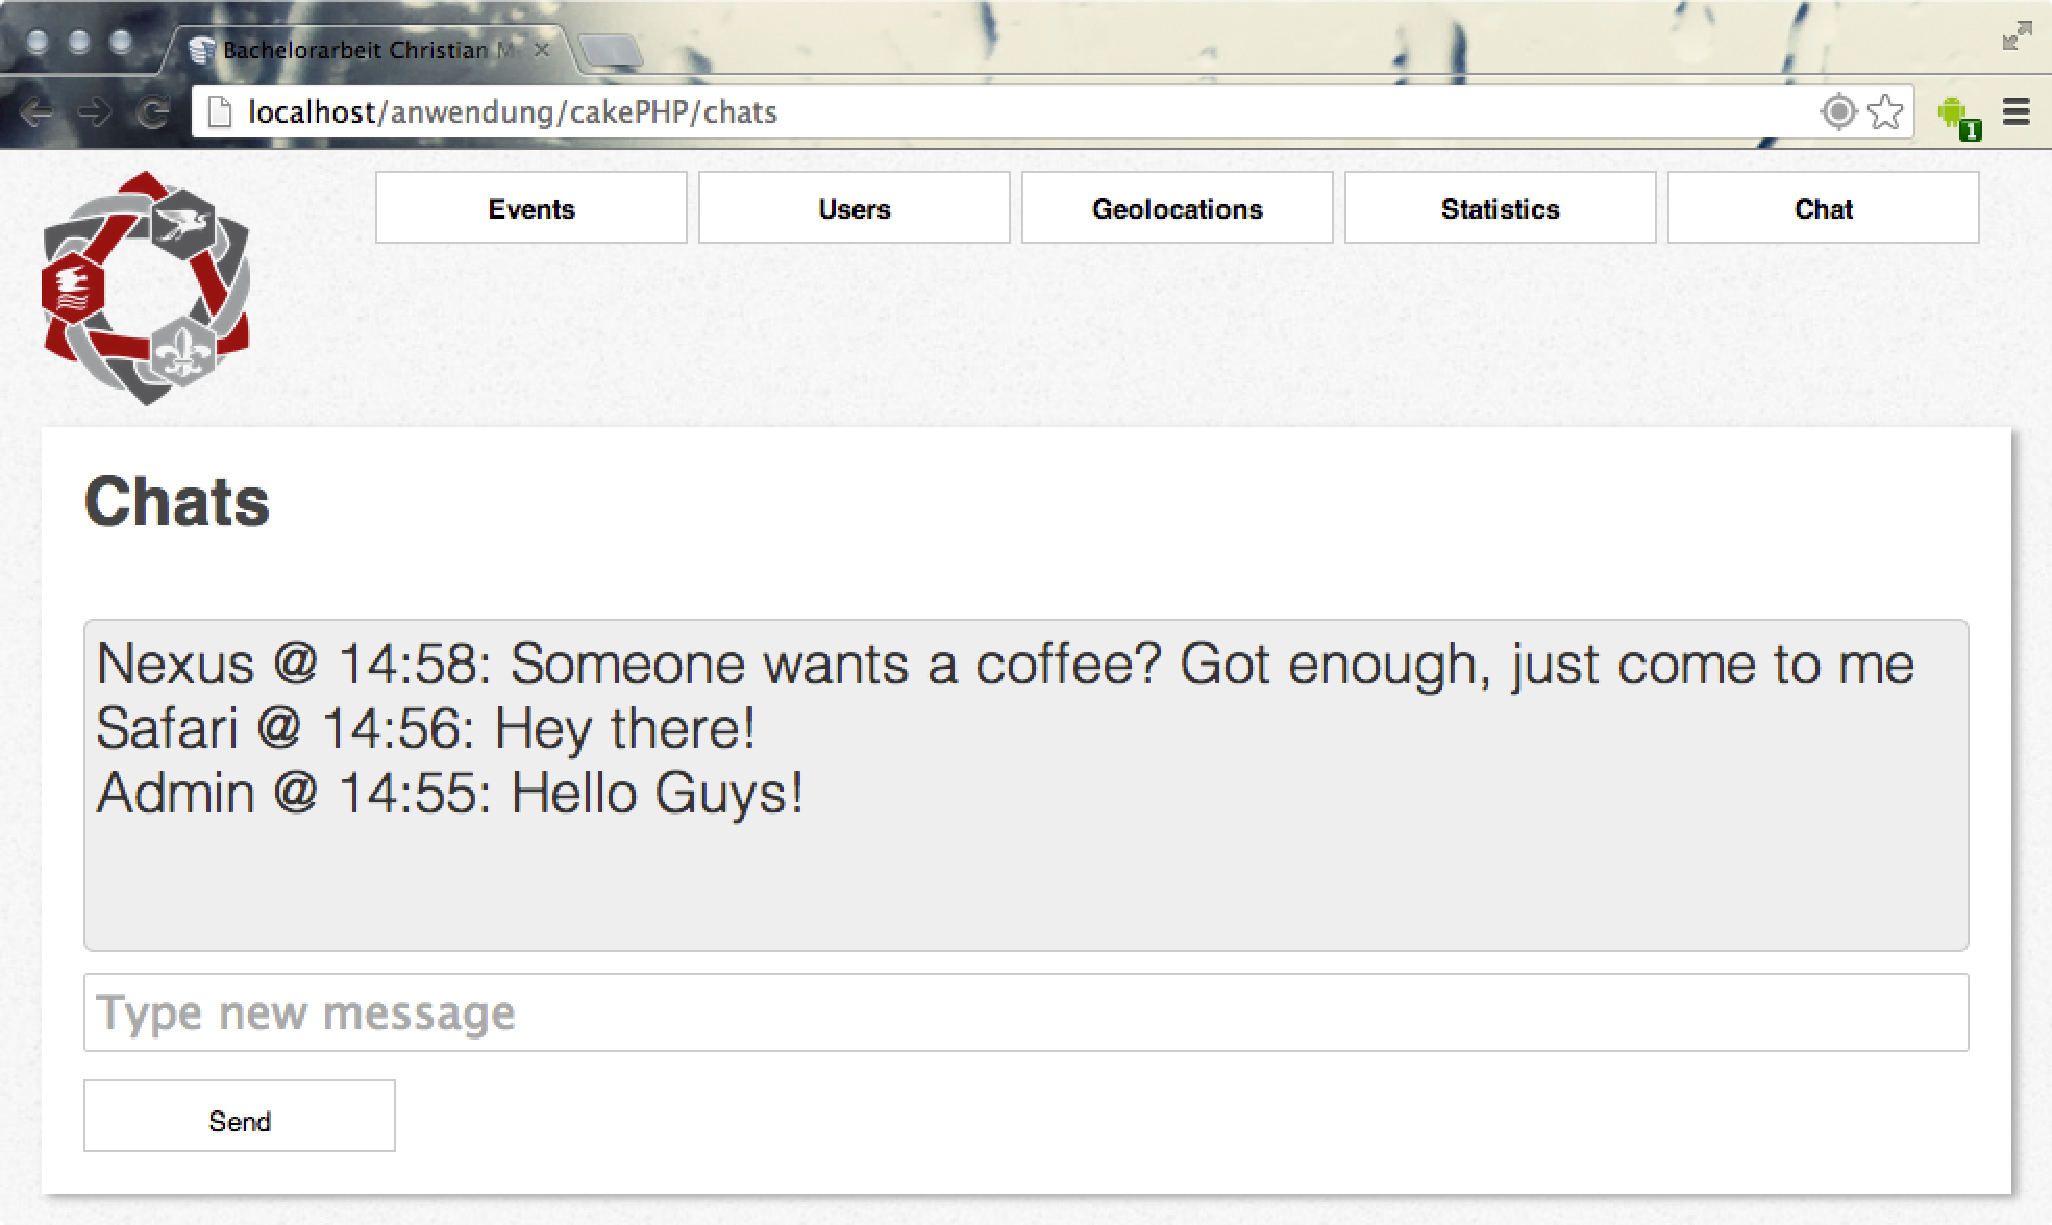
\includegraphics[width=15cm]{fig/screenshot_chat}
	\caption[Beispielansicht der Chats]{Getestet unter OS X 10.8.5., Chrome 29: Chatverlauf von drei verschiedenen Benutzern}
\end{figure}

Hierbei wird wieder Publish / Subscribe verwendet: Befindet sich ein Endgerät gerade im View des Chats, so abonniert die Webanwendung automatisch den Chat beim WebSocket Server und erhält dadurch alle eingehenden Nachrichten.

%%%%%%%%%%%%%%%%%%%%%%%%%%%%%%%%%%%%%%%%%%%%%%%%%%

\section{PUSH-Benachrichtigungen}
Bei Webanwendungen gibt es noch weitere Einschränkungen. So konnte für diese Arbeit nicht auf die systemeigenen Benachrichtigungsmechanismen zurückgegriffen werden, wie man sie aus nativen Applikationen her kennt. In den aktuellen Versionen aller mobilen Betriebssystemen sind Bereiche für Benachrichtigungen aus den jeweiligen Anwendungen implementiert um dem Benutzer zu signalisieren, dass neue Nachrichten vorliegen. Allerdings darf eine Web-App darauf nicht zugreifen, daher wurden für diese Anwendung eigene Methoden auf Basis von \emph{noty} \cite{noty}, einem jQuery Plugin für Benachrichtigungen, implementiert. Mit dieser Bibliothek wurde eine Benachrichtigungsleiste entwickelt, die am unteren Bildschirmrand Informationen anzeigen kann, wie zum Beispiel die oben angesprochene publish-Benachrichtigung vom WebSocket Server.\par

Auf diese Weise können nun auf allen Plattformen, die JavaScript aktiviert haben, Push-Benachrichtigungen angezeigt werden, wenn relevante Informationen über die WebSockets an das Endgerät gelangen.

%%%%%%%%%%%%%%%%%%%%%%%%%%%%%%%%%%%%%%%%%%%%%%%%%%

\section{Statistiken}
Da eine Auswertung der eingegebenen Daten für Veranstaltungen unabdinglich ist, wurde ein weiterer Controller implementiert, welcher sämtliche speziellen Felder der Events aus der Datenbank abfragt und diesen dann die Werte der einzelnen Benutzer zuweist.\par

Im View wird dann eine grafische Auswertung gestartet, die mit Hilfe von \emph{Google Charts} \cite{google:charts} ansehnliche Graphen mit JavaScript generiert, wo es Sinn ergibt und vergleichbare Werte von den Benutzern hinterlegt wurden. Außerdem gibt es allgemeine Statistiken, die die Veranstaltungen untereinander vergleichen und man so einen schnellen Überblick über die angelegten Events erhält.